\begin{figure}[h!]
    \centering
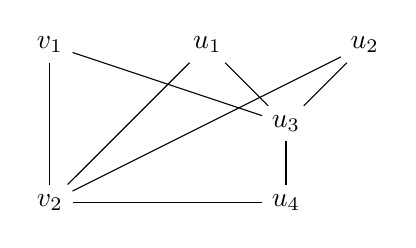
\begin{tikzpicture}
    \node (v1) at (0, 2) {\(v_1\)};
    \node (v2) at (0, 0) {\(v_2\)};
    \draw (v1) -- (v2);
    \node (u1) at (2, 2) {\(u_1\)};
    \node (u2) at (4, 2) {\(u_2\)};
    \node (u3) at (3, 1) {\(u_3\)};
    \node (u4) at (3, 0) {\(u_4\)};
    \draw (u1) -- (u3);
    \draw (u2) -- (u3);
    \draw (u4) -- (u3);
    \draw (v1) -- (u3);
    \draw (v2) -- (u1);
    \draw (v2) -- (u2);
    \draw (v2) -- (u4);
\end{tikzpicture}
\caption{\(\Theta_4\)}
\label{fig:Theta_4}
\end{figure}

\begin{thm}
    If \(\DConf_3(\Gamma)\) is a surface then \(\Gamma\) is either \(K_5\) or the \(\Theta_4\) graph.
\end{thm}
\begin{proof}
    Let \(v_1\) and \(v_2\) be adjacent vertices in \(\Gamma\).
    First, suppose \(\Gamma - \{v_1, v_2\}\) is a \(3\)-cycle, then \(\Gamma\) has \(5\) vertices.
    If \(\Gamma\) is not \(K_5\) then there are two vertices: \(v_i\), and \(u_1\) in \(\Gamma - \{v_1, v_2\}\)
    such that they are not connected by an edge in \(\Gamma\).
    Let \(u_2\) and \(u_3\) be the other two vertices in \(\Gamma - \{v_1, v_2\}\).
    Notice that \(\Gamma - \{u_2, u_3\}\) cannot be either a \(3\)-cycle nor a \(Y\)-graph.

    Suppose instead that \(\Gamma - v_1 v_2\) is a \(Y\)-graph, then \(\Gamma\) has \(6\) vertices.
    Since \(\Gamma\) is connected there exists at least one edge in \(\Gamma\) connecting \(v_1 v_2\) to \(\Gamma - v_1 v_2\).
    We then have one of the following in Figure \ref{fig:edgeygraphconnections}.
    \begin{figure}[h!]
        \centering
        \begin{tikzpicture}
            \node (v1) at (0, 2) {\(v_1\)};
            \node (v2) at (0, 0) {\(v_2\)};
            \draw (v1) -- (v2);
            \node (u1) at (2, 2) {\(u_1\)};
            \node (u2) at (4, 2) {\(u_2\)};
            \node (u3) at (3, 1) {\(u_3\)};
            \node (u4) at (3, 0) {\(u_4\)};
            \draw (u1) -- (u3);
            \draw (u2) -- (u3);
            \draw (u4) -- (u3);
            \draw (v1) -- (u1);
        \end{tikzpicture}
        \quad
        \begin{tikzpicture}
            \node (v1) at (0, 2) {\(v_1\)};
            \node (v2) at (0, 0) {\(v_2\)};
            \draw (v1) -- (v2);
            \node (u1) at (2, 2) {\(u_1\)};
            \node (u2) at (4, 2) {\(u_2\)};
            \node (u3) at (3, 1) {\(u_3\)};
            \node (u4) at (3, 0) {\(u_4\)};
            \draw (u1) -- (u3);
            \draw (u2) -- (u3);
            \draw (u4) -- (u3);
            \draw (v1) -- (u3);
        \end{tikzpicture}
        \caption{Possible ways to connect an edge to a \(Y\)-graph}
        \label{fig:edgeygraphconnections}
    \end{figure}

    Suppose that there is an edge in \(\Gamma\) between \(v_1\) and \(u_1\).
    Applying Lemma \ref{lem:is_surface_Y} to \(\Gamma - \{u_3, u_4\}\), we see there must be an edge
    connecting \(v_1\) and \(u_2\) in \(\Gamma\).
    Applying Lemma \ref{lem:is_surface_Y} to \(\Gamma - \{u_1, u_3\}\), there must be an edge between
    \(v_1\) and \(u_4\) in \(Gamma\).
    Finally, applying Lemma \ref{lem:is_surface_Y} to \(\Gamma - \{v_1, u_1\}\), there must must be
    an edge between \(v_2\) and \(u_2\).
    So in this case, \(\Gamma\) must have \(\Theta_4\) as a subgraph.

    Suppose instead that there is an edge in \(\Gamma\) between \(v_1\) and \(u_3\).
    Applying Lemma \ref{lem:is_surface_Y} to \(\Gamma - \{u_3, u_4\}\),
    we have two subcases.
    \begin{enumerate}
        \item There are edges \(v_1 u_1\) and \(v_1 u_2\) in \(\Gamma\).
        \item There are edges \(v_2 u_1\) and \(v_2 u_2\) in \(\Gamma\).
    \end{enumerate}
    In the second subcase if we apply Lemma \ref{lem:is_surface_Y} to \(\Gamma - \{u_1, u_3\}\),
    we see there must be an edge between \(v_1\) and \(u_4\) in \(\Gamma\).
    So, in this subcase, \(\Gamma\) must have \(\Theta_4\) as a subgraph.
    Suppose the first subcase is true, then applying Lemma \ref{lem:is_surface_Y} to \(\Gamma - \{u_2, u_3\}\),
    it follows that there is an edge between \(v_1\) and \(u_4\) in \(\Gamma\).
    Applying Lemma \ref{lem:is_surface_Y} to \(\Gamma - \{v_1, u_3\}\),
    we have two possibilities.
    \begin{enumerate}
        \item \(v_2\) is the center of the \(Y\)-graph \(\Gamma - \{v_1, u_3\}\).
        \item \(v_2\) is not the center of the \(Y\)-graph \(\Gamma - \{v_1, u_3\}\).
    \end{enumerate}
    If \(v_2\) is the center, then there must be edges \(v_2 u_1\), \(v_2, u_2\), \(v_2 u_4\) in \(\Gamma\).
    Putting particles at the vertices \(v_2\), \(u_2\), and \(u_4\), each of these particles can move
    simultaneously to \(u_1\), \(v_1\), and \(u_3\) respectively.
    This results in \((v_2, u_2, u_4)\) forming the corner of a \(3\)-cube in the configuration space
    contradicting that \(\DConf_3(\Gamma)\) is a surface.

    So, suppose that \(v_2\) is not the center of the \(Y\)-graph. Let \(u_i\) be the center of the \(Y\)-graph.
    Then, there must be an edge connecting \(v_2\) to \(u_i\).
    Putting particles at the vertices \(v_2\), \(u_j\), and \(u_k\) where \(j \neq i\) and \(k \neq i\),
    each of these particles can move simultaneously to \(u_i\), \(v_1\), and \(u_3\) respectively.
    Similarly this results in \((v_2, u_2, u_4)\) forming the corner of a \(3\)-cube in the configuration space.
    Therefore, \(\Gamma\) must have \(\Theta_4\) as a subgraph.

    It remains to show that \(\Gamma\) must equal \(\Theta_4\). Since \(\Gamma\) has \(\Theta_4\) as a subgraph
    if \(\Gamma\) is not \(\Theta_4\) this is equivalent to assuming there is at least one additional edge in \(\Theta_4\).
    So, if we just look at adding in one additional edge we have two possibilities (up to isomorphism).
    \begin{enumerate}
        \item There is an edge between \(v_2\) and \(u_3\).
        \item There is an edge between \(u_1\) and \(u_2\).
    \end{enumerate}
    In the second case, since \(\Gamma - \{u_1, u_2\}\) contains a \(4\)-cycle, Lemma \ref{lem:is_surface_Y} immediately fails.
    So suppose that there is an edge between \(v_2\) and \(u_4\).
    Applying Lemma \ref{lem:is_surface_Y} to \(\Gamma - \{v_2, u_4\}\), we see there must be additional edges to make \(\Gamma - \{v_2, u_3\}\)
    a \(Y\)-graph.
    There are two possibilities.
    \begin{enumerate}
        \item \(v_1\) is the center of the \(Y\)-graph \(\Gamma - \{v_2, u_3\}\).
        \item \(u_i\) is the center of the \(Y\)-graph \(\Gamma - \{v_2, u_3\}\) for some \(i \neq 3\).
    \end{enumerate}
    In either case there must be some edge connecting \(v_1\) to \(u_j\) for some \(j \neq 3\).
    Without a loss of generality suppose \(j = 1\).
    Then, immediately one can see that Lemma \ref{lem:is_surface_Y} fails for \(\Gamma - \{u_3, u_4\}\)
    as what remains contains a \(3\)-cycle.
    Therefore \(\Gamma\) must be \(\Theta_4\).
\end{proof}

\begin{thm}
    If \(\DConf_n(\Gamma)\) is a surface and \(n > 3\), then \(n = 4\) and \(\Gamma = K_{3,3}\).
\end{thm}
\begin{proof}
    Let \(v_1\) and \(v_2\) be adjacent vertices in \(\Gamma\).
    Since \(n > 3\), Lemma \ref{lem:is_surface_2} guarantees that \(\Gamma - \{v_1, v_2\}\) cannot be a \(Y\)-graph.
    So, \(\Gamma - \{v_1, v_2\}\) must be an \(n\)-cycle.
    Let \(u_1, u_2, \cdots, u_n\) be the vertices on the \(n\) cycle.
    Since \(\Gamma\) is connected there must be some edge connecting either \(v_1\) or \(v_2\) to some \(u_i\).
    Without a loss of generality suppose that \(v_1\) is connected to \(u_1\).
    If \(n > 4\) apply Lemma \ref{lem:is_surface_C} to \(\Gamma - \{v_1, u_1\}\) and see that
    \(u_2\) and \(u_n\) must connect to \(v_2\) in \(\Gamma\).
    Now put particles at each vertex in \(\{v_1, u_1, u_2, \cdots, u_n\}\setminus\{u_4\}\).
    As the particle at \(u_3\) moves to \(u_4\), any one of the particles at \(v_1\), \(u_2\), or \(u_n\) 
    can move to \(v_2\). These particles movements correspond to a book in the configuration space
    whose spine corresponds to the movement of the particle at \(u_3\) to \(u_4\).
    Therefore \(n\) must equal \(4\).
    See Figure \ref{fig:edge4cycle} for the current situation.
    Applying Lemma \ref{lem:is_surface_C} to \(\Gamma - \{v_1, u_1\}\), there must be an edges
    \(v_2 u_2\) and \(v_2 u_4\) in \(\Gamma\).
    Applying Lemma \ref{lem:is_surface_C} to \(\Gamma - \{v_2, u_2\}\), there must be an edge connecting \(v_1\)
    and \(u_2\).
    Therefore \(\Gamma\) must have \(K_{3,3}\) as a subgraph.

    Suppose that \(\Gamma\) was not \(K_{3,3}\).
    Then there is at least one additional edge.
    Without a loss of generality suppose this edge is \(u_2, u_4\).
    Then, \(\Gamma - \{v_1, u_3\}\) contains a \(3\)-cycle contradicting Lemma \ref{lem:is_surface_C}.
    Hence \(\Gamma\) must be \(K_{3,3}\).
    \begin{figure}[h!]
        \centering
        \begin{tikzpicture}
            \node (v1) at (0, 2) {\(v_1\)};
            \node (v2) at (0, 0) {\(v_2\)};
            \node (u1) at (3, 2) {\(u_1\)};
            \node (u2) at (2, 1) {\(u_2\)};
            \node (u4) at (4, 1) {\(u_4\)};
            \node (u3) at (3, 0) {\(u_3\)};
            \draw (v1) -- (v2);
            \draw (u1) -- (u2);
            \draw (u2) -- (u3);
            \draw (u3) -- (u4);
            \draw (u4) -- (u1);

            \draw (v1) -- (u1);
        \end{tikzpicture}
        \caption{Edge connected to \(4\)-cycle}
        \label{fig:edge4cycle}
    \end{figure}

    \begin{figure}[h!]
        \centering
        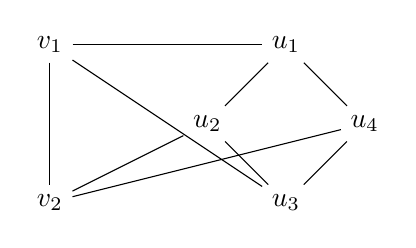
\begin{tikzpicture}
            \node (v1) at (0, 2) {\(v_1\)};
            \node (v2) at (0, 0) {\(v_2\)};
            \node (u1) at (3, 2) {\(u_1\)};
            \node (u2) at (2, 1) {\(u_2\)};
            \node (u4) at (4, 1) {\(u_4\)};
            \node (u3) at (3, 0) {\(u_3\)};
            \draw (v1) -- (v2);
            \draw (u1) -- (u2);
            \draw (u2) -- (u3);
            \draw (u3) -- (u4);
            \draw (u4) -- (u1);
            \draw (v1) -- (u1);
            \draw (v1) -- (u3);
            \draw (v2) -- (u2);
            \draw (v2) -- (u4);
        \end{tikzpicture}
        \label{fig:K3,3}
        \caption{\(K_{3,3}\)}
    \end{figure}

\end{proof}